\documentclass[12pt,a4paper]{article}
\usepackage[utf8]{inputenc}
\usepackage[french]{babel}
\usepackage[T1]{fontenc}
\usepackage{amsmath}
\usepackage{amsfonts}
\usepackage{amssymb}
\usepackage{graphicx}
\usepackage[left=2cm,right=2cm,top=2cm,bottom=2cm]{geometry}
\usepackage[thinspace,thinqspace,amssymb]{SIunits}
\usepackage{eurosym}

\usepackage{hyperref}
\hypersetup{
    colorlinks=true,
    urlcolor=theme
}

\title{Mise en perspective didactique d'un dossier de recherche}
\author{\textbf{Rémi Metzdorff}}
\date{Concours externe spécial de l'agrégation de physique-chimie option physique Session 2020}
%\date{2020}

\renewcommand{\d}{\mathrm{d}}
\newcommand{\uroc}{\micro RoC}

%%%%%%%%%%%%%%%%%%%%%%%%%%%%%%  For CV  %%%%%%%%%%%%%%%%%%%%%%%%%%%%%%
\usepackage{array}
%\newcolumntype{L}[1]{>{\raggedright\let\newline\\\arraybackslash\hspace{0pt}}m{#1}}
%\newcolumntype{C}[1]{>{\centering\let\newline\\\arraybackslash\hspace{0pt}}m{#1}}
%\newcolumntype{R}[1]{>{\raggedleft\let\newline\\\arraybackslash\hspace{0pt}}m{#1}}
%%%%%%%%%%%%%%%%%%%%%%%%%%%%%%%%%%%%%%%%%%%%%%%%%%%%%%%%%%%%%%%%%%%%%%

\usepackage{xcolor}
\definecolor{theme}{RGB}{56,115,179}
\usepackage[font=small]{caption}

%%%%%%%%%%%%%%%%%%%%%%%%%%%%%%%%%%%%%%%%%%%%%%%%%%%%%%%%%%%%%%%%%%%%%%
\usepackage[framemethod=tikz]{mdframed}

\mdfdefinestyle{s_mep}{
	linecolor=theme!,
	outerlinewidth=3pt,
	frametitlerule=false,
	topline=false,
	bottomline=false,
	rightline=false,
	backgroundcolor=white,
	innertopmargin=5pt,
	roundcorner=0pt,
	%skipabove=5pt,
	skipbelow=5pt
}
\newmdenv[style=s_mep]{mep_env}

\newenvironment{mep}{%\stepcounter{exa}%
%\newenvironment{myenv}{\begin{adjustwidth}{2cm}{}}{\end{adjustwidth}}
\addcontentsline{ldf}{figure}{0}%
\begin{mep_env}
\small}
{\end{mep_env}}
%%%%%%%%%%%%%%%%%%%%%%%%%%%%%%%%%%%%%%%%%%%%%%%%%%%%%%%%%%%%%%%%%%%%%%

%\footnote{Abbott \textit{et al.}, Observation of Gravitational Waves from a Binary Black Hole Merger, \textit{Phys. Rev. Lett.} \textbf{116}, (2016)}

%\vspace*{20pt}
%\begin{center}
%\begin{large}
%\textsc{Mise en perspective didactique d'un dossier de recherche}
%\end{large}
%\vspace{10pt}
%Concours externe spécial de l'agrégation de physique-chimie, option physique -- 2020
%\vspace{20pt}
%\textbf{Rémi Metzdorff}
%\end{center}

\begin{document}

\maketitle
%\tableofcontents

\section{Parcours universitaire et scientifique}

\noindent
\begin{tabular*}{\textwidth}{p{0.12\textwidth}<{\raggedleft}p{0.83\textwidth}}
\textcolor{theme}{\rule{0.12\textwidth}{2.5mm}} &
\large\textcolor{theme}{Formation et doctorat} \vspace{3pt} \\
2019--2020 &
\textbf{Préparation à l'agrégation} au centre de Montrouge (ENS, Sorbonne Université, Univresité Paris-Saclay).\\
2015--2019 &
\textbf{Doctorat :} Thèse réalisée au sein de l'équipe \og optomécanique et mesures quantiques \fg{} du laboratoire Kastler-Brossel (LKB, Paris) sous la direction de Pierre-François Cohadon, intitulée \textit{Refroidissement de résonateurs macroscopiques proche de leur état quantique fondamental}, soutenue le 23 juillet 2019. \\
2014--2015 &
\textbf{Master 2 :} Parcours LuMI (Lumière, matière, interactions) du master OMP (Optique, matière, plasma) de l'université Pierre et Marie Curie (UPMC, Paris).
Stage de recherche au LKB avec Pierre-François Cohadon (6 mois) sur l'étude des pertes dans des cavités Fabry-Perot de grande finesse. \\
2013--2014 &
\textbf{Master 1 :} Parcours physique générale du master Physique et applications de l'UPMC (Paris).
Stage au LKB avec Pierre Cladé (4 mois) sur le développement de collimateurs compacts pour les faisceaux d'un piège magnéto-optique sur une expérience de métrologie. \\
2012--2013 &
\textbf{Licence 3 :} Parcours physique-chimie de l'UPMC (Paris). \\
2010--2012 &
\textbf{CPGE :} PCSI et PC$^*$ au lycée Louis-le-Grand (Paris). \vspace{10pt} \\

\textcolor{theme}{\rule{0.12\textwidth}{2.5mm}} &
\large\textcolor{theme}{Enseignements, diffusion et vulgarisation} \vspace{3pt} \\
2015--2018 & \textbf{Missions d'enseignement :} ($\unit{64}{h\per an}$)
\begin{itemize}
\item travaux pratiques d'électromagnétisme (L1) ;
\item travaux dirigés et travaux pratiques de physique expérimentale (L2-L3) : programmation, électronique, Arduino ;
\item travaux pratiques d'optique (M1) : laser, diode laser.
\end{itemize}\\
\vspace{-8mm} 2019 &
\vspace{-8mm} \textbf{Un chercheur, Une manip :} présentations au Palais de la découverte autour de la détection d'ondes gravitationnelles.\\
2017 &
\textbf{Olympiades de physique :} conférence sur la découverte des ondes gravitationnelles devant les candidats.\\
2017 &
\textbf{E=M6 :} casser un verre avec la voix, recherche et mise en place de l'expérience, présentation lors du tournage.\\
2015--2018 &
\textbf{Fête de la science :} conférence sur la détection d'ondes gravitationnelles, animations et présentation du LKB au grand public, notamment à travers des visites et quelques expériences : résonance optique du sodium, interférence en comptage de photons, etc\\
2012--2018 &
\textbf{Aïkido :} enseignant au cours enfant (8 à 15 ans). 
\end{tabular*}

\section{Refroidissement vers l'état quantique fondamental}

\subsection{Mesure de déplacements et optomécanique}
\label{sec:intro}

\subsubsection{Les mesures de déplacements et leurs applications}

\begin{figure}[b]
\center
%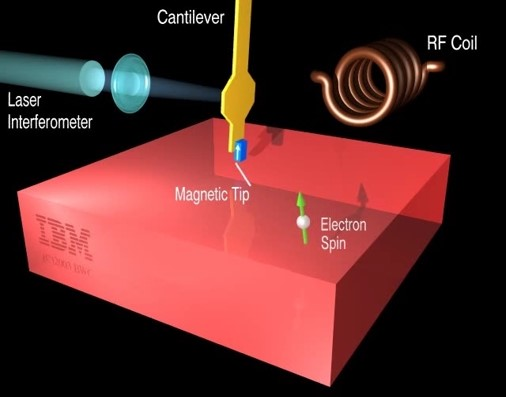
\includegraphics[height=90pt]{figures/AFM_RM.jpg}
%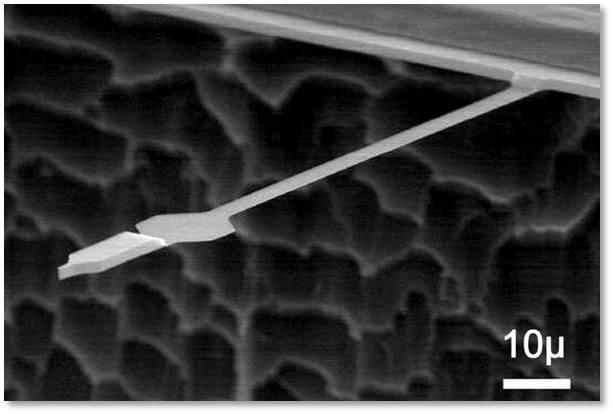
\includegraphics[height=90pt]{figures/AFM_quantilever.png}
%\hfill
%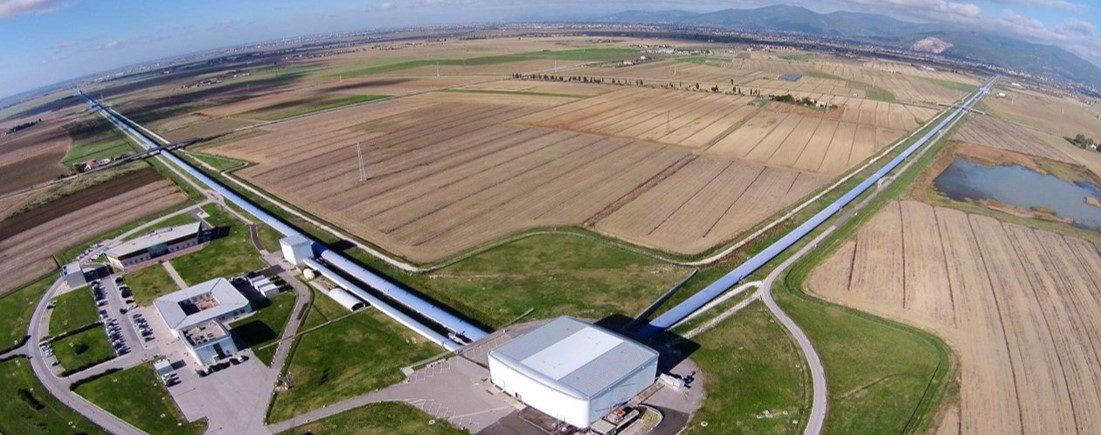
\includegraphics[height=90pt]{figures/virgo.jpg}
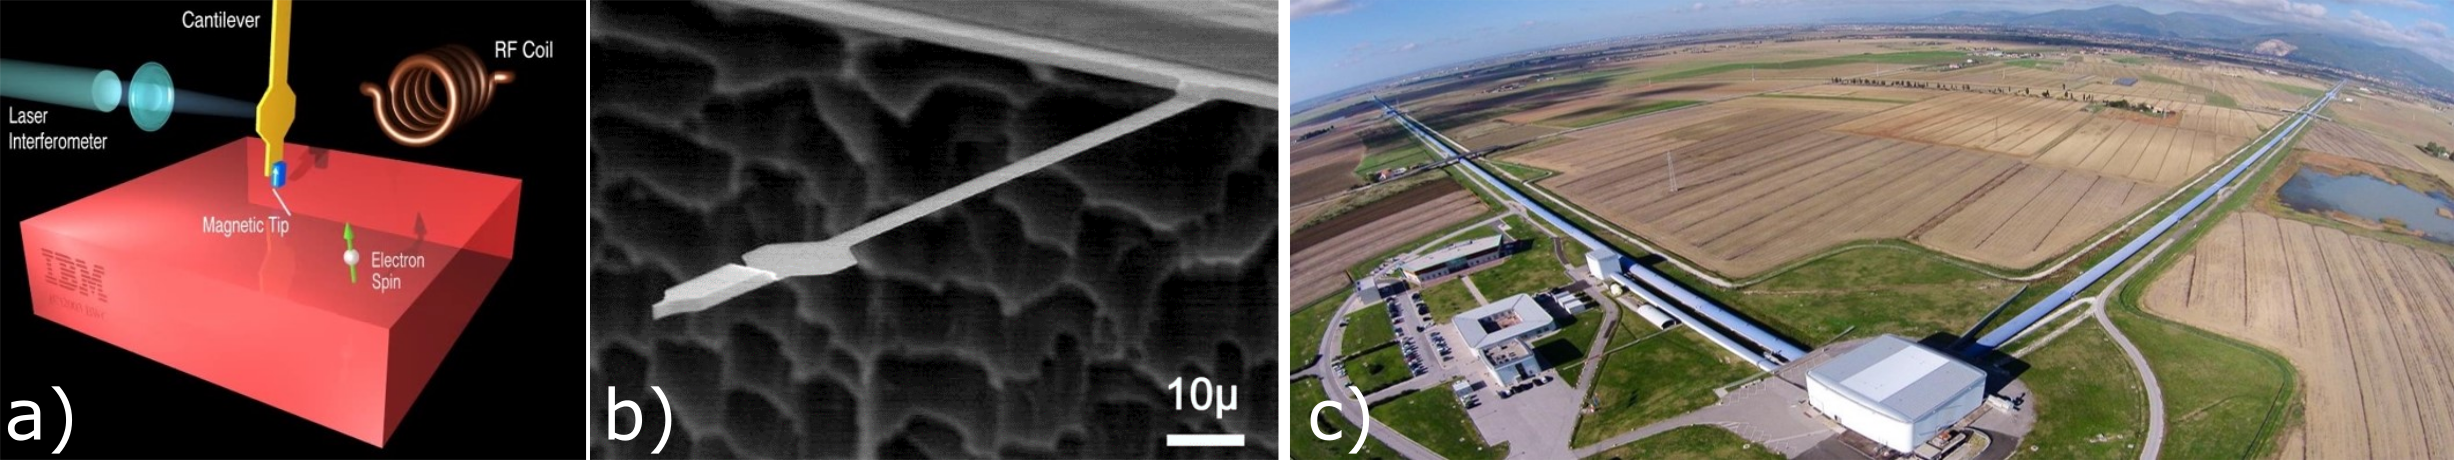
\includegraphics[height=90pt]{figures/displacement.png}
\caption{Les mesures de déplacements sont utiles aussi bien pour sonder la matière que pour des observations astronomiques.
(a) Résonance magnétique par mesure de force (D. Rugar, 2004), capable de détecter des spins uniques exerçant sur (b) le micro-levier une force de l'ordre de $\unit{10^{-18}}{\newton}$, associée à un déplacement de $\unit{10^{-10}}{\meter}$.
(c) Interféromètre gravitationnel Virgo avec ses bras de \unit{3}{\kilo\meter}, qui atteint maintenant une sensibilité relative inférieure à $10^{-22}$.}
\label{fig:displacement_measurement}
\end{figure}

Les mesures de déplacements sont parmi les mesures les plus sensibles réalisées à ce jour.
À l'échelle astronomique, on souhaite par exemple connaître la distance (et la vitesse) séparant plusieurs objets afin de déterminer la vitesse d'expansion de l'univers.
À l'échelle microscopique, ces mesures permettent d'élaborer des capteurs variés, très sensibles mais de dimensions très faibles : accéléromètres et gyroscopes en mesurant le déplacement d'une masse test, microscope à force atomique en observant la déviation d'un micro-levier à proximité de la surface d'un échantillon,~etc.
 
De nombreux dispositifs de mesure de déplacements utilisent les propriétés remarquables de la lumière.
La \textit{mesure absolue} de la distance Terre-Lune découle par exemple de la détermination du temps de vol d'impulsions lumineuses avec des incertitudes relatives de l'ordre de $10^{-9}$.
Le développement de techniques interferométriques autorise par ailleurs les \textit{mesures relatives} les plus sensibles réalisées à ce jour (Fig.~\ref{fig:displacement_measurement}).

Un des succès majeurs de l'interférométrie optique est la détection des ondes gravitationnelles par les interféromètres des projets Virgo (Cascina, Italie) et LIGO (Hanford et Livingston, États-Unis).
Les développements considérables des dernières décennies ont en effet permis, cent ans après leur prédiction par A. Einstein, l'observation directe d'ondes gravitationnelles issues de la coalescence de deux trous noirs
\footnote{Abbott \textit{et al.}, Observation of Gravitational Waves from a Binary Black Hole Merger, \textit{Phys. Rev. Lett.}, (2016)}.
L'amplitude relative maximale du signal mesuré sur Terre était alors proche de $10^{-21}$, soit un déplacement équivalent mille fois plus petit que la taille d'un proton, ce qui en faisait le signal le plus faible jamais détecté associé à l'évènement le plus violent jamais observé.

Les détecteurs d'ondes gravitationnelles sont des interféromètres de Michelson géants dont les bras sont des cavités Fabry-Perot pour augmenter l'effet d'un petit déphasage : la longueur des bras de Virgo est de \unit{3}{\kilo\meter} avec des cavités de finesse 50.
Le passage d'une onde gravitationnelle introduit un déphasage qui peut être mesuré à la sortie de l'appareil comme des variations de l'intensité lumineuse transmise par l'interféromètre.

\subsubsection{L'optomécanique : entre limite de sensibilité...}

Dans le cas des interféromètres gravitationnels, toute perturbation du détecteur produit un bruit qui dégrade la sensibilité de la mesure s'il n'est pas causé par le passage d'une onde gravitationnelle.
La distribution spectrale de ces bruits dépend de leur nature et leur influence dépend de l'intervalle de fréquences sur lequel est réalisée la mesure.
Par exemple, l'agitation thermique microscopique engendre un mouvement aléatoire macroscopique de la surface des optiques du détecteur.
C'est le mouvement brownien qu'il est possible d'atténuer en utilisant des matériaux et des géométries adaptés.
La réduction des bruits classiques est telle que les bruits quantiques de phase et d'intensité liés au laser lui-même deviennent limitants.

Le \textit{bruit quantique de phase} influence directement la mesure puisque, contrairement au bruit classique, les fluctuations quantiques de phase sont décorrélées entre les deux bras de l'interféromètre.
Le \textit{bruit quantique d'intensité} a deux conséquences : un bruit direct sur l'intensité mesurée à la sortie du détecteur et des fluctuations de la force de pression de radiation qui s'exerce sur les miroirs de l'interféromètre et agit sur leur position.
C'est l'action en retour de la mesure, prédite dès les années 80, qui a contribué à fonder les recherches sur l'interaction entre un rayonnement électromagnétique et un mouvement mécanique : l'optomécanique.

Dans un interféromètre de Michelson, le déplacement $\delta x$ d'un miroir est associé à un déphasage
\begin{equation}
\delta \varphi = \delta \varphi ^\mathrm{phase} _\mathrm{q} + \frac{4\pi}{\lambda} ( \delta x + \delta x ^\mathrm{rad} _\mathrm{q} + \delta x_\mathrm{c}),
\label{eq:disp}
\end{equation}
où $\delta \varphi ^\mathrm{phase} _\mathrm{q}$ est le bruit quantique de phase, $\delta x ^\mathrm{rad} _\mathrm{q}$ le bruit de position associé au bruit quantique d'intensité et où $\delta x_\mathrm{c}$ regroupe les bruits classiques.
L'amplitude du bruit quantique de phase est inversement proportionnelle à l'amplitude du champ lumineux.
En revanche, l'amplitude du bruit quantique de pression de radiation est proportionnelle à l'amplitude du champ et est modulée par la réponse mécanique du système.
Si l'on augmente l'intensité du laser, le bruit de phase diminue mais le bruit de pression de radiation augmente.
Pour chaque fréquence de mesure, il existe donc une puissance laser optimale pour laquelle les bruits quantiques de phase et de pression de radiation sont égaux : c'est la \textit{limite quantique standard}.

\subsubsection{... Et contrôle d'oscillateurs mécaniques}

Même si la pression de radiation peut dégrader la sensibilité des mesures interférométriques, on peut l'exploiter pour contrôler les degrés de liberté mécaniques d'un système mécanique.
Au cours des vingt dernières années, de nombreux systèmes optomécaniques ont ainsi été développés : micro-capteurs de force, de masse, de température, transducteurs optique-microonde, etc.
Une application fondamentale de ces systèmes est l'observation d'effets quantiques sur des objets de plus en plus massifs et c'est dans cette démarche que s'inscrit mon sujet de thèse, avec le \textit{refroidissement d'un oscillateur mécanique macroscopique dans son état quantique fondamental}.

Un tel refroidissement a été réalisé pour la première fois en 2011 sur un oscillateur de faible masse ($m_\mathrm{eff} = \unit{50}{pg}$) couplé à une cavité microonde\footnote{Teufel \textit{et al.}, Sideband cooling of micromechanical motion to the quantum ground state, \textit{Nature}, (2011)}.
L'enjeu de ma thèse repose sur l'utilisation de systèmes \emph{macroscopiques}, de masse effective proche de \unit{100}{\micro\gram}, soit trois ordres de grandeur de plus que les autres expériences actuelles.
Cette masse est choisie proche de la masse de Planck ($m_\mathrm{P}=\unit{22}{\micro\gram}$) au delà de laquelle les effets de décohérence liés à la gravité deviennent significatifs, marquant ainsi la frontière entre les \og mondes \fg{} quantiques et classiques. 
Le système dans son état fondamental permettrait en outre d'explorer les limites quantiques de sensibilité des mesures de petits déplacements liées au bruit de pression de radiation, tout en restant beaucoup plus compact que les interféromètres gravitationnels et leurs miroirs ($m_\mathrm{eff}\approx\unit{50}{\kilo\gram}$).
En effet, il est possible d'observer le bruit quantique de pression de radiation pour des puissances optiques modérées une fois l'état fondamental atteint.

Le refroidissement se fait en utilisant les techniques de l'optomécanique en cavité, pour lesquelles il convient de disposer de \textit{bons} oscillateurs mécaniques : nous les décrirons dans un premier temps.
Pour mesurer leurs déplacements avec précision, ces oscillateurs sont utilisés comme l'un des miroirs d'une cavité optique de grande finesse.
Nous détaillerons ensuite l'utilisation du couplage optomécanique pour le refroidissement de l'oscillateur en cavité.
Nous exposerons finalement les principaux résultats obtenus au cours de la thèse.
Ils seront brièvement mis en perspective dans le cadre de l'amélioration de la sensibilité des détecteurs d'ondes gravitationnelles.

\subsection{Les oscillateurs mécaniques}
\label{sec:mechanical_oscillators}

\begin{figure}[b!]
\center
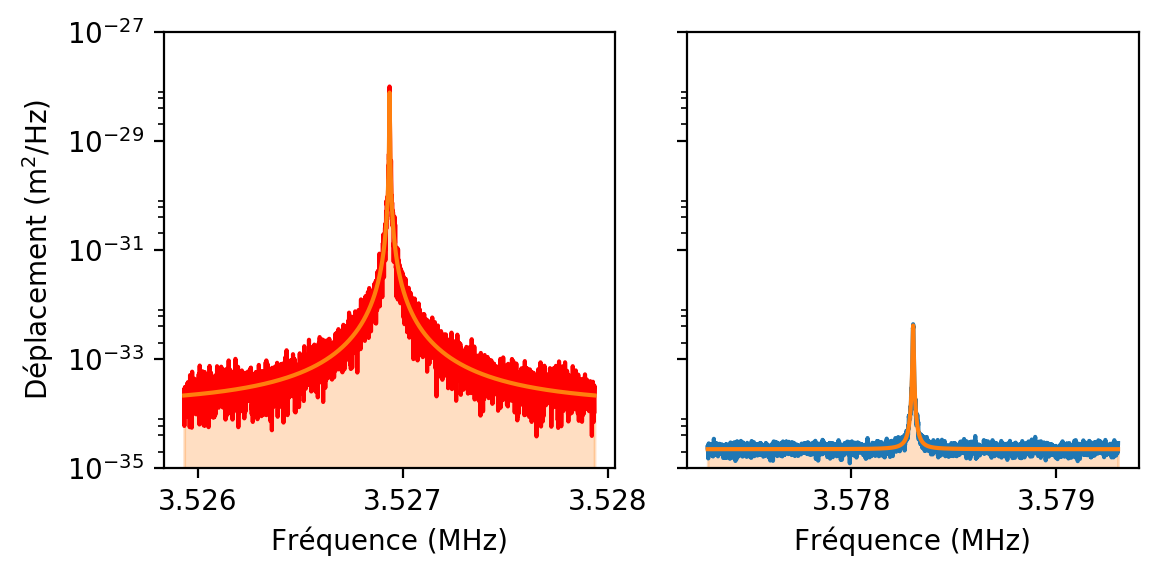
\includegraphics[scale=0.75]{figures/thermal_peak_def_filled.png}
\caption{Spectres des fluctuations de position d'un oscillateur (micro-pilier) dues au mouvement brownien de l'oscillateur.
Sa masse effective est déduite d'une mesure à température ambiante (à gauche) : l'oscillateur est à l'équilibre avec son environnement ($T=T_\mathrm{env}$) et la température $T_\mathrm{env}$ est obtenue grâce à une thermistance.
Lors du refroidissement (à droite), cette même mesure donne la température $T$ de l'oscillateur puisque $m_\mathrm{eff}$ ne change pas. 
Le déplacement est exprimé en $\meter\squared{.}\hertz^{-1}$ car on s'intéresse non à l'amplitude mais à la densité spectrale de puissance du bruit de position.}
\label{fig:thermal_noise}
\end{figure}

Pour de faibles perturbations, le comportement des oscillateurs mécaniques est très bien décrit par un système \{masse, ressort\} amorti à un degré de liberté soumis à des forces extérieures de résultante $F_\mathrm{ext}$, si bien que l'équation du mouvement s'écrit
\begin{equation}
m_\mathrm{eff}\left[\frac{\d ^2 x(t)}{\d t^2} + \Gamma_m \frac{\d  x(t)}{\d t} +  \Omega_m^2 x(t)\right] = F_\mathrm{ext}(t),
\label{eq:eq_of_motion}
\end{equation}
où $m_\mathrm{eff}$ est la masse effective, $\Omega_m$ la pulsation propre et $\Gamma_m$ l'amortissement.
Le comportement fréquentiel se déduit dans l'espace de Fourier de la susceptibilité mécanique $\chi[\Omega]$ de l'oscillateur :
\begin{equation}
\chi[\Omega] = \frac{1}{m_\mathrm{eff}[(\Omega_m^2-\Omega^2)-i\Gamma_m\Omega]},
\end{equation}
telle que $x[\Omega] = \chi[\Omega]F_\mathrm{ext}[\Omega]$.

L'agitation thermique microscopique se traduit au niveau macroscopique comme une excitation aléatoire du mode propre de l'oscillateur à l'origine du mouvement brownien décrit par la théorie de Langevin.
%où le terme de dissipation $\Gamma_m$ est responsable d'un couplage de l'oscillateur à son environnement assimilé à un bain thermique à la température $T_\mathrm{env}$.
%Il en résulte une force fluctuante $F_\mathrm{T}[\Omega]$ dont le spectre est lié à la partie imaginaire de la susceptibilité mécanique par le théorème de fluctuation-dissipation.
Dans le cas où la dissipation est faible ($\Gamma_m \ll \Omega_m$), on montre que le spectre de déplacement de l'oscillateur est bien approché par une lorentzienne de largeur $\Gamma_m$ centrée sur la pulsation propre.
On utilise donc des oscillateurs avec des facteurs de qualité mécaniques $Q=\Omega_m/\Gamma_m$ très élevés ($Q>10^6$).
Par ailleurs, l'intégrale du spectre est liée à la température $T$ de l'oscillateur : elle est fonction directe du rapport $T/m_\mathrm{eff}$.
Connaissant sa masse effective, \textit{une acquisition du mouvement brownien de l'oscillateur permet donc de mesurer sa température} et inversement (Fig.~\ref{fig:thermal_noise}).

La description classique ne permet cependant pas d'expliquer le comportement de l'oscillateur aux très basses températures.
Il est nécessaire d'utiliser un modèle quantique, où le hamiltonien du système est celui d'une masse $m_\mathrm{eff}$ dans un puits de potentiel harmonique à une dimension, de pulsation $\Omega_m$.
La résolution de l'équation de Schrödinger conduit à une quantification des niveaux d'énergie $E_n = \hbar\Omega_m (n_\mathrm{T}+\frac{1}{2})$, où $n_\mathrm{T}$ est le nombre de phonons qui caractérise l'état de l'oscillateur.
Le niveau d'occupation du système est donné par la statistique de Bose-Einstein :
\begin{equation}
n_\mathrm{T} = \left[ e^\frac{T_Q}{T} -1\right]^{-1},
\label{eq:phonon_number}
\end{equation}
où la température quantique $T_Q$ est définie par $T_Q = \hbar\Omega_m/k_B$.
En particulier, l'énergie minimale du système dans son état fondamental n'est pas nulle et induit un bruit de position appelé \og fluctuations de point zéro\fg{}.
Il s'agit donc pour nous de refroidir un oscillateur mécanique à une température $T$ pour laquelle $n_\mathrm{T} < 1$, c'est-à-dire $T \lesssim T_Q$.

\begin{figure}
\center
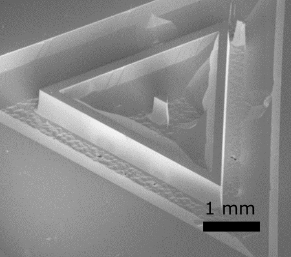
\includegraphics[height=90pt]{figures/micropillar.png}
\hfill
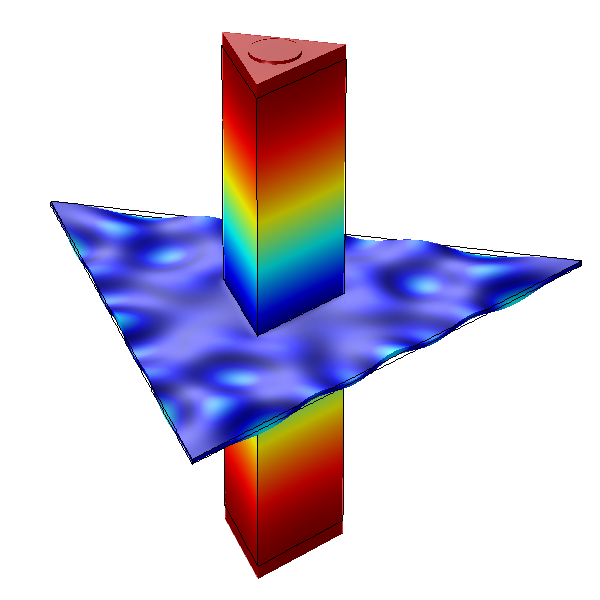
\includegraphics[height=90pt]{figures/micropillar_disp.png}
\hfill
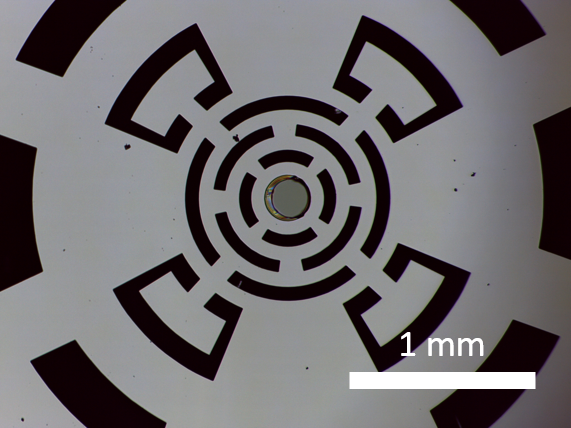
\includegraphics[height=90pt]{figures/microwheel.png}
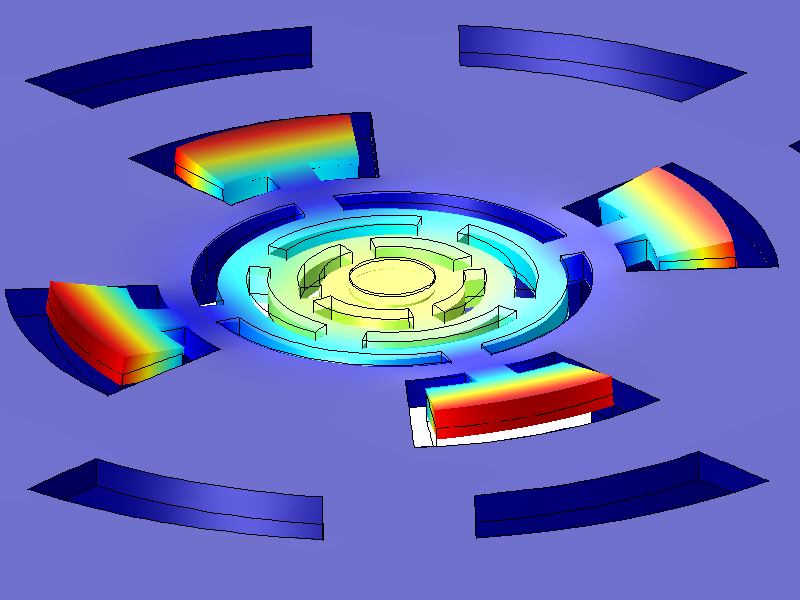
\includegraphics[height=90pt]{figures/microwheel_disp.png}
\caption{À gauche : image obtenue par microscopie électronique d'un micro-pillier et simulation par élément fini (COMSOL) du mode propre de compression utilisé.
À droite : image obtenue par microscopie optique d'un micro-disque et simulation du mode propre utilisé.
Le code couleur correspond au déplacement de la structure, du bleu au rouge, le rouge correspondant au déplacement maximal.}
\label{fig:resonators}
\end{figure}

Au cours de ma thèse, j'ai utilisé deux types d'échantillons (Fig.~\ref{fig:resonators}) :
\begin{itemize}
\item un micro-pilier en quartz de \unit{1}{\milli\meter} de long, de section triangulaire de \unit{240}{\micro\meter} de côté, micro-fabriqué à l'ONERA (Paris) et en collaboration avec le LMA (Lyon).
Il est suspendu en son milieu par une membrane d'environ \unit{10}{\micro\meter} d'épaisseur et on dépose un miroir de haute réflectivité sur l'une de ses extrémités.
Avec $m_\mathrm{eff}=\unit{33{,}5}{\micro\gram}$ et $\Omega_m=2\pi\times\unit{3{,}6}{\mega\hertz}$, on a $T_{Q}^\mathrm{pilier} = \unit{200}{\micro\kelvin}$ avec des facteurs de qualité allant jusqu'à $10^7$ ;
\item un micro-disque en silicium obtenu en collaboration avec l'UniFI (Italie) d'environ $\unit{200}{\micro\meter}$ de diamètre, sur lequel est déposé un miroir de très haute réflectivité.
Avec $m_\mathrm{eff}=\unit{112}{\micro\gram}$ et $\Omega_m=2\pi\times\unit{280}{\kilo\hertz}$, on a $T_{Q,\mathrm{disque}} = \unit{10}{\micro\kelvin}$ avec $Q\approx10^6$.
\end{itemize}
Les propriétés mécaniques $\Omega_m$ et $\Gamma_m$ des échantillons sont obtenues en étudiant leur réponse à une excitation forcée par une cale piézoélectrique.

\subsection{Une cavité optique pour augmenter la sensibilité}
\label{sec:cavity}

On mesure les déplacements de l'oscillateur par interférométrie optique : la réflexion d'un faisceau laser sur le miroir de l'oscillateur s'accompagne d'un déphasage $\delta\varphi$ qui dépend du déplacement $\delta x$ du miroir.
La sensibilité $\delta\varphi / \delta x$ de la mesure dépend de la détection employée.
Dans le cas d'un interféromètre de Michelson dont l'un des bras porte le miroir mobile (Fig.~\ref{fig:detection_scheme},~(a)), la sensibilité vaut $4\pi/\lambda$ et ne dépend que de la longueur d'onde du laser.
Dans une cavité de finesse $\cal{F}$ (Fig.~\ref{fig:detection_scheme},~(b)), la lumière effectue environ $\cal{F}$ allers-retours ce qui permet d'amplifier l'effet du déplacement d'un de ses miroirs.
Si la cavité est résonante avec le laser, le déphasage devient
\begin{equation}
\delta \varphi = 8{\cal{F}}\frac{\delta x}{\lambda}.
\end{equation}
Le déphasage est ensuite converti en variation d'intensité détectable par une photodiode en faisant interférer ce faisceau signal avec un faisceau de référence (Fig.~\ref{fig:detection_scheme},~(c)).

Pour les caractérisations préliminaires des échantillons, un simple interféromètre de Michelson convient puisqu'on étudie un régime forcé pour lequel l'amplitude des déplacements est grande.
En revanche, pour les mesures de mouvement brownien, la sensibilité de l'interféromètre seul est insuffisante et il est nécessaire d'exploiter la réponse en phase d'une cavité Fabry-Perot dont l'un des miroirs est celui de l'oscillateur mécanique.
On obtient finalement une détection homodyne en remplaçant la photodiode de l'interféromètre par une détection équilibrée, non représentée sur les schémas.
Elle permet d'atténuer fortement les bruits classiques et autorise des mesures limitées par les bruits quantiques. 

\begin{figure}
\center
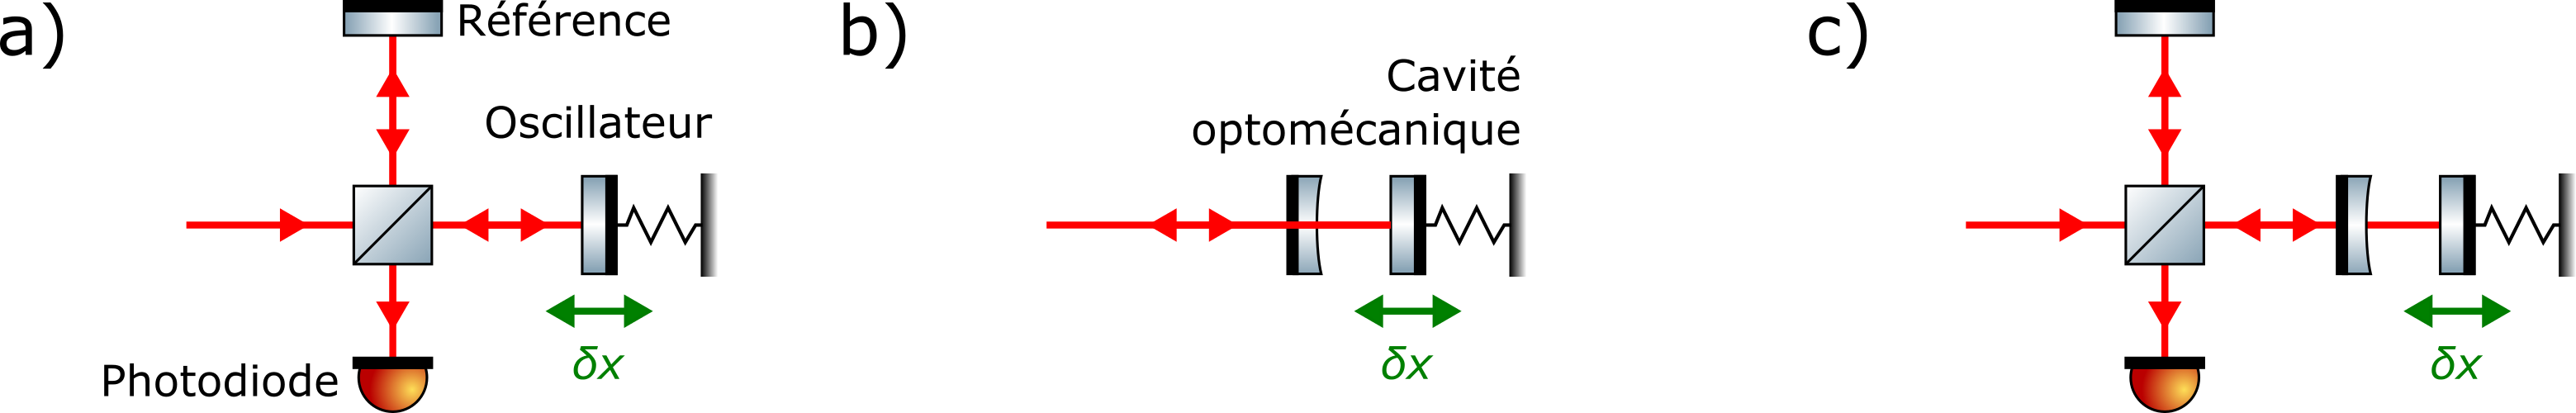
\includegraphics[height=75pt]{figures/detection_scheme.png}

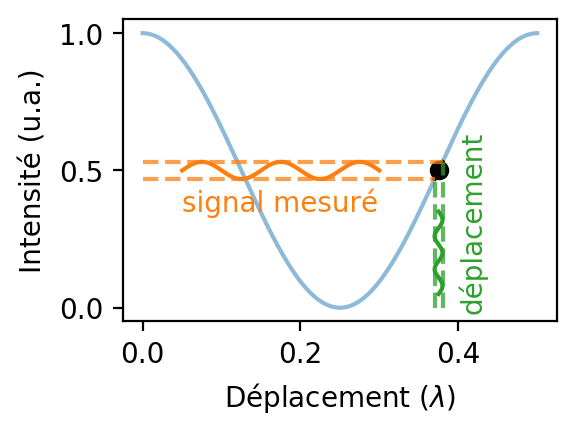
\includegraphics[scale=0.75]{figures/michelson_response.png}
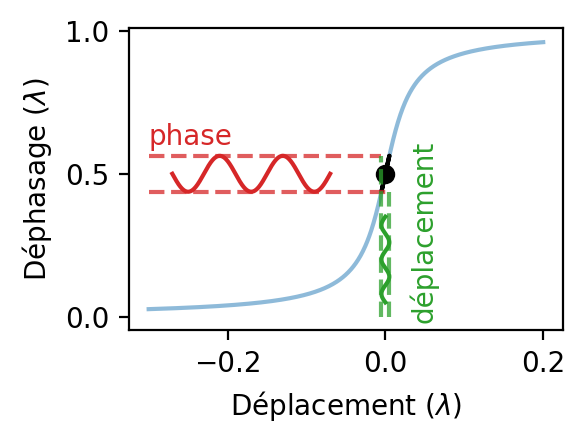
\includegraphics[scale=0.75]{figures/cavity_phase_response_ppt.png}
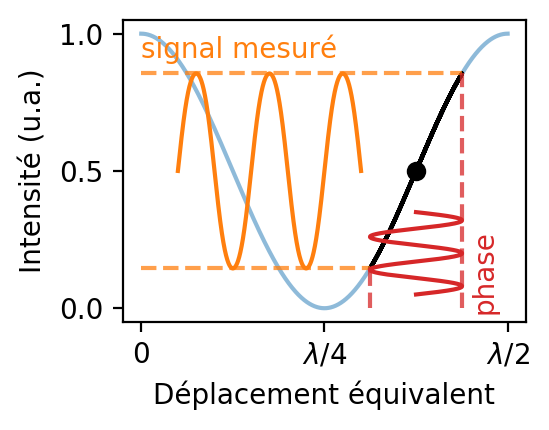
\includegraphics[scale=0.75]{figures/michelson_and_cavity_response.png}
\caption{Schéma simplifié des dispositifs interférométriques utilisés pour la mesure de petits déplacements avec un laser de longueur d'onde $\lambda$.
(a) Mesure de l'intensité transmise par un interféromètre de Michelson.
(b) L'utilisation d'une cavité Fabry-Perot résonante (${\cal{F}}=20$) augmente l'effet d'un petit déplacement et améliore la sensibilité de l'interféromètre (c).
Les graphes indiquent la réponse de la détection (en bleu) en fonction de la position de l'oscillateur et l'allure du signal mesuré (en orange) lors d'un petit déplacement $\delta x$ (en vert) au voisinage du point de fonctionnement optimal (en noir) où la sensibilité est maximale.}
\label{fig:detection_scheme}
\end{figure}

Compte tenu de la faible dimension des miroirs plans déposés sur les oscillateurs mécaniques, il est nécessaire d'utiliser à l'entrée de la cavité un miroir d'un rayon de courbure de l'ordre du millimètre (\uroc).
Avec un laser $\mathrm{CO_2}$, j'ai fabriqué par photoablation des structures concaves d'environ $\unit{200}{\micro\meter}$ de diamètre, possédant des rayons de courbure variés.
Un dépôt diélectrique de couches de silice $\mathrm{SiO_2}$ et d'oxyde de tantale $\mathrm{Ta_2O_5}$ réalisé au Laboratoire des matériaux avancés (Lyon) permet ensuite d'obtenir des miroirs ayant une transmission bien contrôlée entre 0 et $\unit{120}{ppm}$ pour nos échantillons.
J'ai ensuite réalisé un ensemble de pièces mécaniques en cuivre de haute pureté (Fig.~\ref{fig:cavity}) permettant un assemblage et un alignement rapide d'une cavité d'environ $\unit{100}{\micro\meter}$ de longueur, constituée d'un oscillateur et d'un \uroc.
Sa conception est soumise à de nombreuses contraintes liées à son utilisation dans le cryostat à dilution et à la nécessité de l'asservir en longueur pour la maintenir résonante avec le laser.

\begin{figure}
\center
%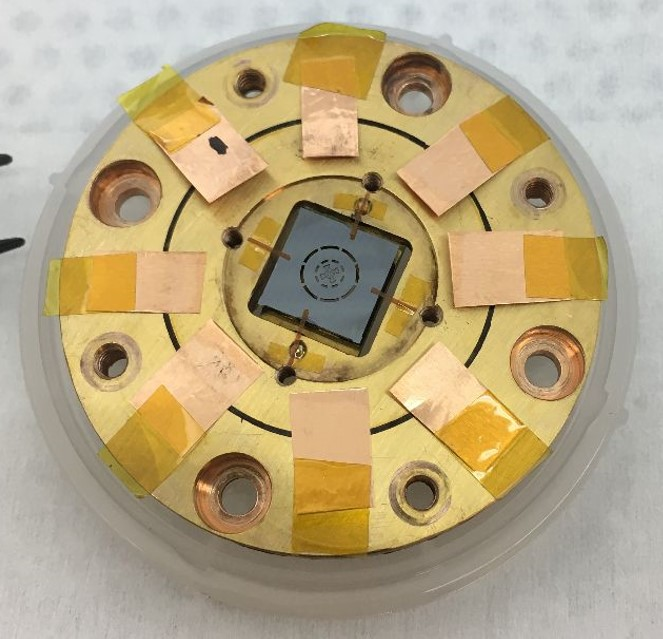
\includegraphics[height=130pt]{figures/cavity_microwheel.jpg}
%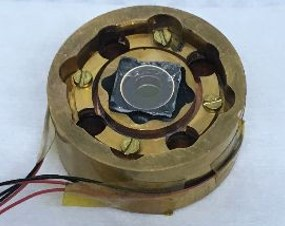
\includegraphics[height=130pt]{figures/cavity_uroc.jpg}
%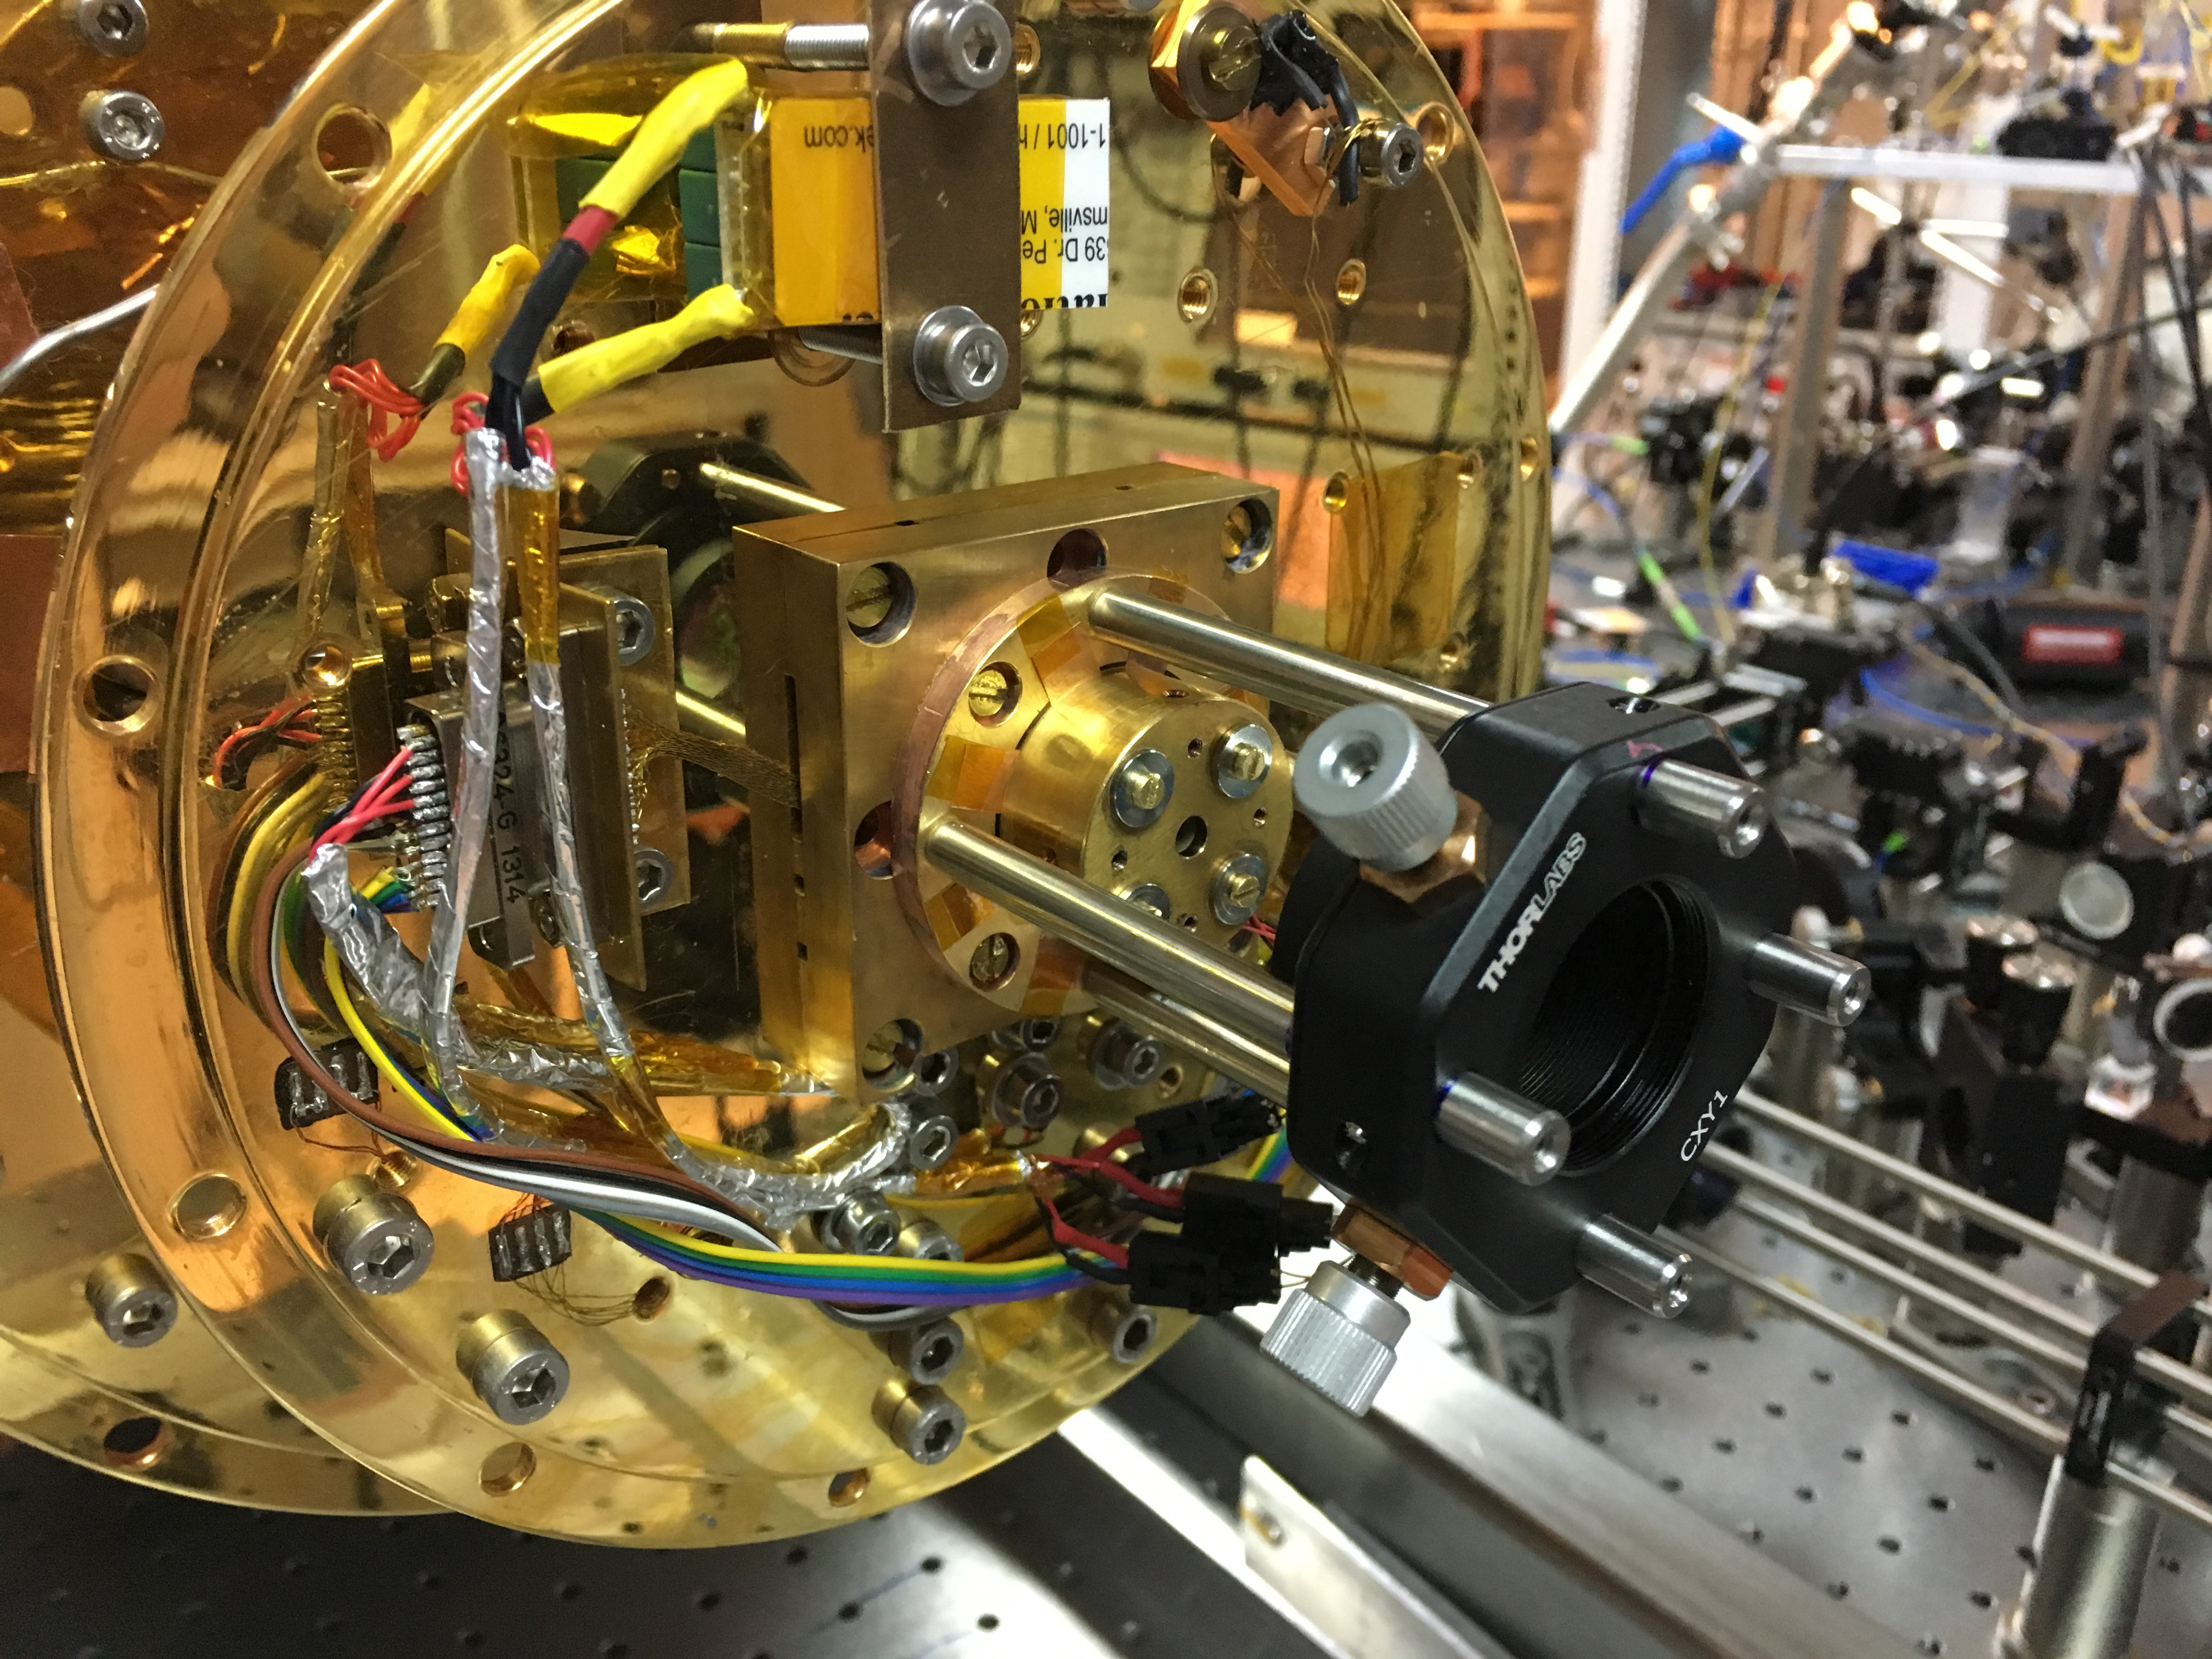
\includegraphics[height=130pt]{figures/IMG_1766.JPG}
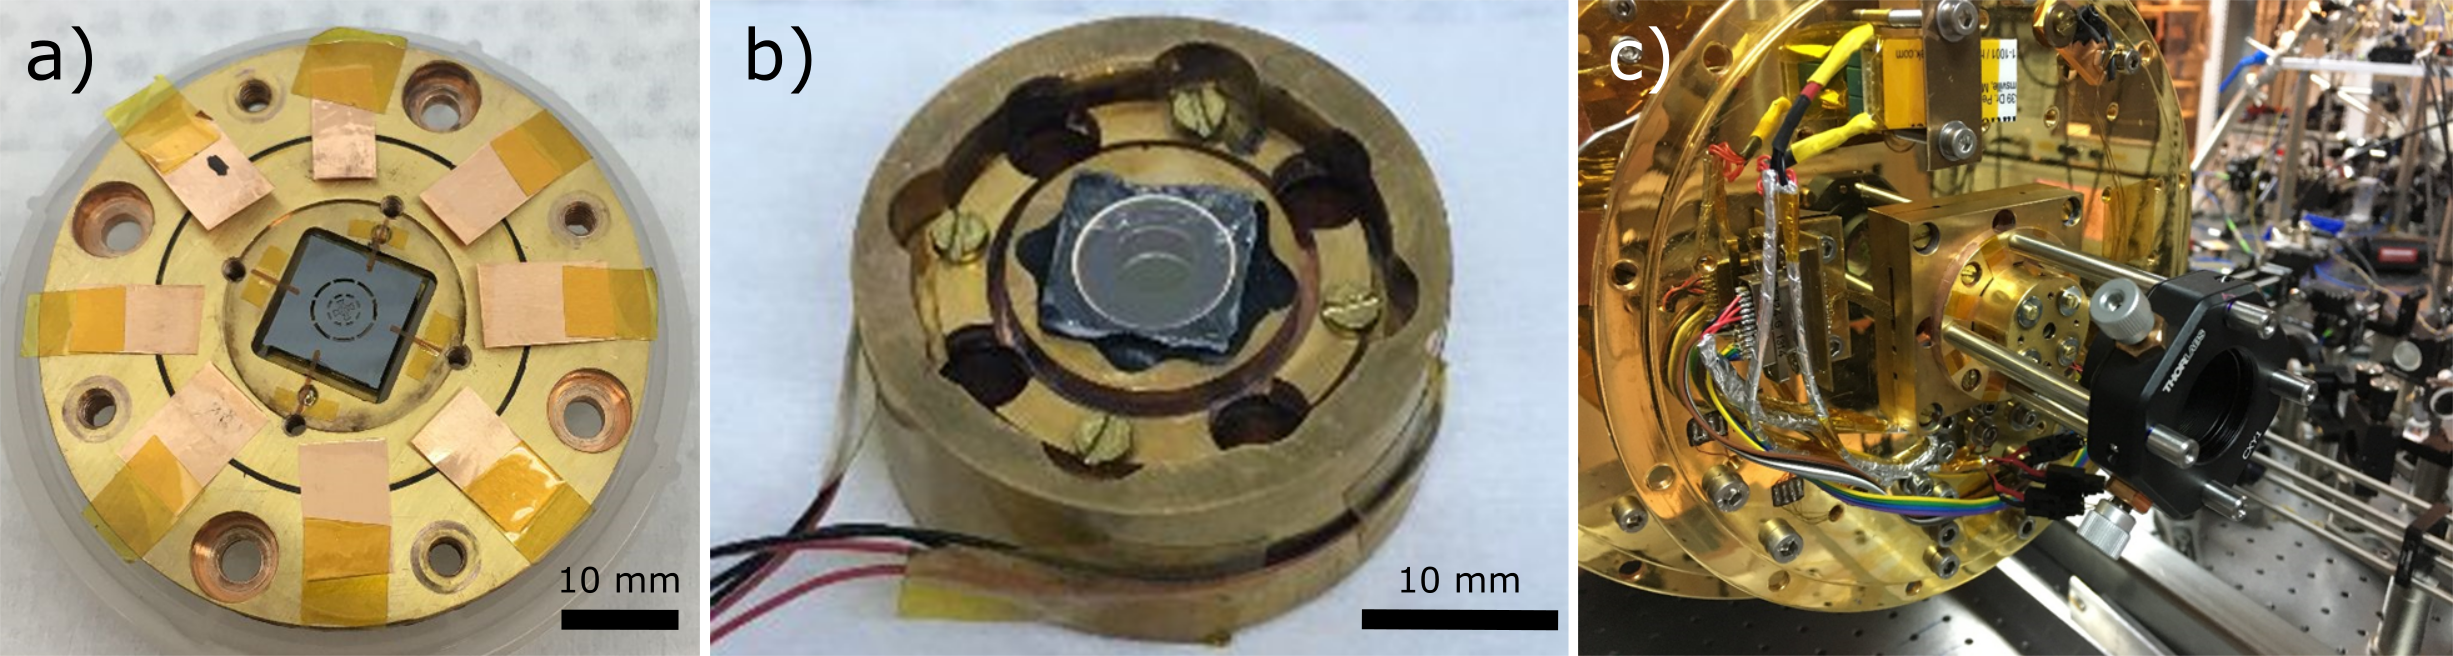
\includegraphics[height=129pt]{figures/optomechanical_cavity.png}
\caption{Cavité optomécanique formée par (a) l'oscillateur mécanique, ici un micro-disque, et (b) le miroir de couplage (\uroc).
Les câbles permettent de contrôler les cales piézoélectriques nécessaires à l'asservissement en longueur de la cavité.
La cavité assemblée (c) est montée sur le dernier étage du cryostat à dilution.
Une lentille de courte focale permet finalement d'adapter le faisceau incident au mode optique fondamental de la micro-cavité.}
\label{fig:cavity}
\end{figure}

\subsection{Couplage optomécanique et refroidissement}
\label{sec:optomechanics}

La température à atteindre pour préparer un oscillateur mécanique dans son état quantique fondamental est de l'ordre de \unit{100}{\micro\kelvin} avec nos échantillons : $T_{Q,\mathrm{pilier}} = \unit{200}{\micro\kelvin}$ et $T_{Q,\mathrm{disque}} = \unit{10}{\micro\kelvin}$.
Il faut donc le refroidir de plus de six ordres de grandeur par rapport à la température ambiante.
Dans un premier temps, l'ensemble de la cavité est refroidi jusqu'à \unit{30}{\milli\kelvin} dans un cryostat à dilution fonctionnant avec un mélange $\mathrm{^4He/^3He}$.
Les techniques propres à l'optomécanique en cavité\footnote{Aspelmeyer \textit{et al.}, Cavity Optomechanics, \textit{Rev. Mod. Phys.}, (2014)} permettent ensuite de refroidir l'oscillateur mécanique jusqu'aux températures requises.

Si le laser est légèrement désaccordé par rapport à la cavité, une perturbation de sa longueur provoquée par un déplacement du miroir mobile modifie la puissance intracavité, ce qui en retour change la force de pression de radiation exercée sur le miroir : c'est le \textit{couplage optomécanique}.
La modulation de la force de pression de radiation $F_\mathrm{rad}$ est déphasée par rapport aux déplacements du miroir et se décompose en deux termes :
\begin{itemize}
\item l'un en phase avec le déplacement qui s'ajoute à la force de rappel mécanique et modifie simplement la pulsation propre $\Omega_m$ : c'est l'effet de \textit{ressort optique} ;
\item l'autre, en quadrature, est proportionnel à la vitesse du miroir et permet d'obtenir une force analogue à un frottement visqueux associé à un taux de dissipation $\Gamma_\mathrm{opt}$.
\end{itemize}

À la différence de la dissipation mécanique $\Gamma_m$ responsable du mouvement brownien, la dissipation optique $\Gamma_\mathrm{opt}$ se fait sans ajout de bruit thermique, ce qui permet de refroidir l'oscillateur : c'est la \textit{friction froide}.
Sa température effective $T_\mathrm{eff}$ est alors différente de celle de l'environnement $T_\mathrm{env}$ et on montre :
\begin{equation}
T_\mathrm{eff} = T_\mathrm{env} \frac{\Gamma_m}{\Gamma_m+\Gamma_\mathrm{opt}}.
\end{equation}
Cette relation justifie l'utilisation d'oscillateurs avec des grands facteurs de qualité et celle d'un cryostat à dilution pour avoir $T_\mathrm{env}$ aussi faible que possible.
L'auto-refroidissement nécessite \og simplement \fg{} d'asservir la longueur de la cavité pour que $\omega_\mathrm{L} < \omega_\mathrm{cav}$, où $\omega_\mathrm{cav}$ est la pulsation de la cavité et $\omega_\mathrm{L}$ celle du laser\footnote{Si à l'inverse $\omega_\mathrm{L} > \omega_\mathrm{cav}$, $\delta F_{\mathrm{rad}, v}$ correspond à un terme d'amplification ($\Gamma_\mathrm{opt} < 0 $ et $T_\mathrm{eff} > T_\mathrm{env}$), pouvant mener à un système instable si $\Gamma_m + \Gamma_\mathrm{opt} < 0$.}.
Cette technique a permis d'atteindre un taux d'occupation de 20 phonons qui justifie le traitement quantique de l'oscillateur.
Avec cette méthode, le refroidissement est limité par la puissance optique injectable dans la cavité.

\begin{figure}
\center
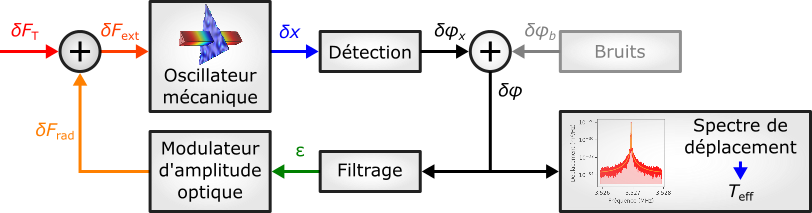
\includegraphics[scale=0.6]{figures/feedback_cooling_v2.png}
\caption{Principe du refroidissement par rétroaction.
La dissipation mécanique $\Gamma_m$ est responsable de la force de Langevin dont les fluctuations $\delta F_\mathrm{T}$ perturbent l'oscillateur.
La détection par interférométrie optique du déphasage $\delta \varphi_x$ associé au déplacement $\delta x$ donne accès à la température de l'oscillateur $T_\mathrm{eff}$ d'après le spectre de ses fluctuations de position.
Après filtrage, on obtient également un signal d'erreur $\epsilon$ qui permet de rétroagir sur l'échantillon par une correction adaptée $\delta F_\mathrm{rad}$ de la force de pression de radiation exercée par le faisceau incident.
La détection est imparfaite : l'ajout de bruit $\delta \varphi_b$ dégrade la sensibilité de mesure et diminue l'efficacité du refroidissement.}
\label{fig:feedback_scheme}
\end{figure}

En plus de la rétroaction passive inhérente au couplage optomécanique, on peut agir activement sur les déplacements du miroir mobile grâce au refroidissement par rétroaction (Fig.~\ref{fig:feedback_scheme}).
La mesure optique de la position de l'oscillateur sert à créer un signal d'erreur grâce auquel on applique une force de frottements visqueux sur le miroir mobile.
Le contrôle du déphasage introduit par la boucle de contrôle permet d'obtenir uniquement le terme de friction froide nécessaire au refroidissement.
La rétroaction peut être appliquée grâce à de nombreux actionneurs, mais dans notre expérience, on utilise un modulateur d'amplitude optique qui agit sur l'intensité du faisceau mesurant les déplacements de l'oscillateur.
La modulation d'amplitude ne perturbe pas la mesure puisqu'il s'agit d'une mesure de phase. 
À puissance optique égale, cette technique est plus efficace que l'auto-refroidissement puisque l'intensité de la rétroaction peut être facilement augmentée en accroissant le gain $g$ de la boucle de contrôle.

Dans le cas d'une mesure parfaite des déplacements du miroir, un accroissement du gain $g$ entraine toujours un refroidissement de l'oscillateur car seul le signal correspondant à ses déplacements est mesuré puis réinjecté dans la boucle.
Dans la réalité, la sensibilité est limitée par les fluctuations de position du miroir d'entrée, le bruit électronique et ultimement, les bruits quantiques.
Il existe donc un gain optimal $g_\mathrm{opt}$ pour lequel le mouvement brownien de l'oscillateur est équivalent au bruit de la mesure.
Pour $g>g_\mathrm{opt}$, le bruit de la mesure perturbe la rétroaction et sa contribution à l'agitation de l'oscillateur provoque une élévation de la température effective : le refroidissement est maximal pour $g=g_\mathrm{opt}$.
La sensibilité des mesures de déplacement est donc l'enjeu majeur pour atteindre l'état quantique fondamental.

\subsection{Principaux résultats obtenus}
\label{sec:results}

Après avoir caractérisé les échantillons mécaniques et réalisé les micro-miroirs de couplage, la cavité optomécanique est alignée et montée dans le cryostat à dilution puis refroidie vers \unit{30}{\milli\kelvin}.
Sa longueur moyenne est asservie sur le laser et on optimise les paramètres de la boucle de contrôle du refroidissement par rétroaction.
Cette phase s'accompagne d'une identification méticuleuse des parasites électroniques, acoustiques et optiques qui compromettent la stabilité de l'expérience pour les atténuer.
On acquiert finalement le spectre des fluctuations de position de l'oscillateur en faisant varier le gain $g$ du refroidissement par rétroaction avec des atténuateurs analogiques.
Les résultats obtenus avec un micro-pilier sont visibles sur la Fig.~\ref{fig:feedback_cooling_pillar}.

Il a ainsi été possible de refroidir le micro-pilier jusqu'à une température effective $T_\mathrm{eff} = \unit{1{,}0\pm 0{,}1}{\milli\kelvin}$, ce qui correspond à un taux d'occupation de $\mathbf{5{,}3 \pm 0{,}5}$ \textbf{phonons}.
Des limitations importantes principalement attribuées à la dégradation progressive de l'échantillon, conduisant notamment à des instabilités photothermiques nous ont conduit à utiliser l'autre type d'oscillateur : le micro-disque.
Avec ces échantillons et en seulement quelques mois, il a été possible d'atteindre une température de \unit{0{,}7\pm 0{,}1}{\milli\kelvin} correspondant à un niveau d'occupation de $\mathbf{55\pm5}$ \textbf{phonons}, cette fois limité par le bruit de détection causé par les fluctuations de position du miroir d'entrée de la cavité.
À température comparable, le niveau d'occupation de l'oscillateur obtenu avec le micro-disque est dix fois plus élevé que celui du micro-pilier car la fréquence du mode propre des micro-disques est dix fois plus faible ($T_Q = \hbar\Omega_m/k_B$).
Ces résultats font état des \textit{taux d'occupation thermique les plus faibles atteints actuellement avec des oscillateurs mécaniques aussi macroscopiques} ($m_\mathrm{eff}\approx\unit{100}{\micro\gram}$). 

\begin{figure}
\center
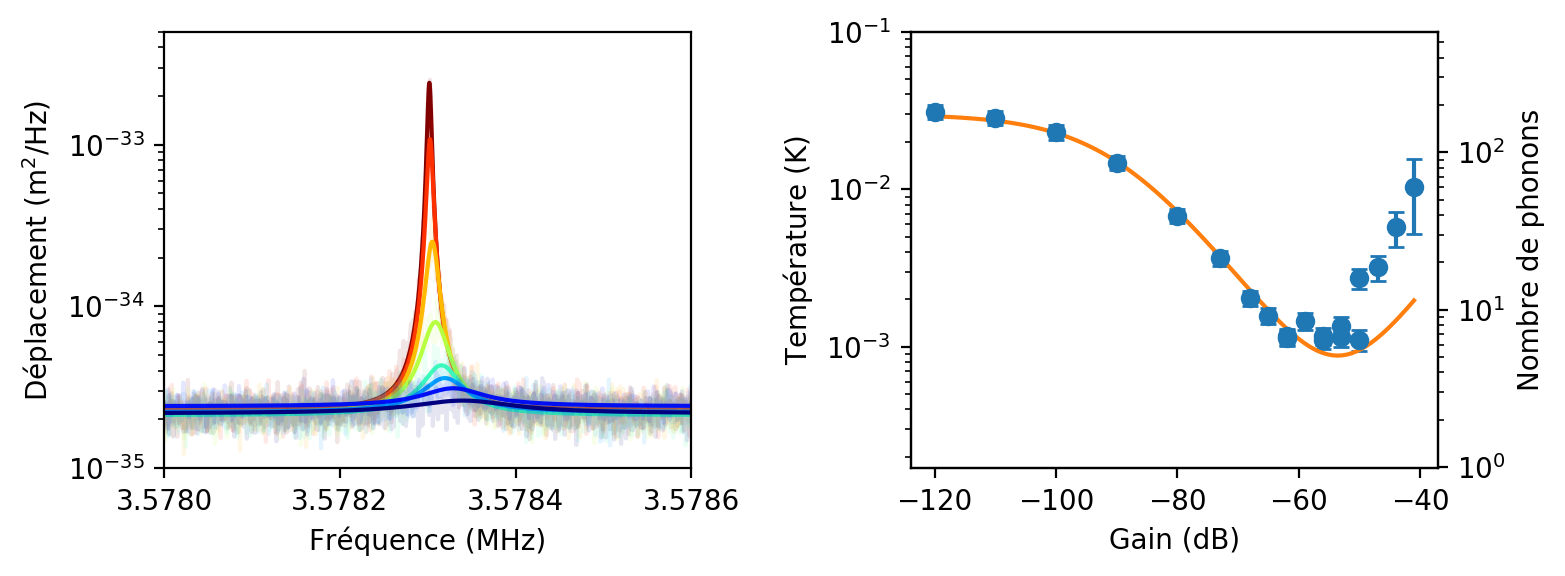
\includegraphics[scale=0.75]{figures/feedback_cooling_6phonons.png}
\caption{Refroidissement d'un micro-pilier proche de son état quantique fondamental.
À gauche : spectres des fluctuations de position obtenus pour différents gains (du rouge pour les gains faibles au violet pour le gain optimal).
Les données expérimentales sont tracées en transparence et l'ajustement lorentzien par le modèle théorique correspond aux courbes pleines.
À droite : températures effectives $T_\mathrm{eff}$ déduites de l'intégrale des courbes précédentes.
La courbe orange correspond au modèle qui tient compte des paramètres de l'expérience.}
\label{fig:feedback_cooling_pillar}
\end{figure}

\subsection{Vers des mesures sous la limite quantique standard}
\label{sec:prospects}

Dans notre expérience, le signal que l'on mesure est associé au mouvement brownien de l'oscillateur, concentré autour de la pulsation mécanique $\Omega_m$.
La limite de sensibilité de la plupart de nos mesures est imposée par le bruit quantique de phase, qui forme le plancher observé vers $\unit{2\times10^{-35}}{\meter\squared{.}\hertz^{-1}}$ sur la Fig.~\ref{fig:feedback_cooling_pillar}.
Compte tenu des puissances optiques utilisées et du niveau d'occupation thermique atteint, le bruit quantique d'intensité ne représente qu'une fraction de l'ordre de \unit{1}{\%} des fluctuations de position mesurées.
Grâce aux développements réalisés sur la cavité optomécanique, une observation du bruit de pression de radiation devrait être possible, notamment en utilisant une puissance optique plus importante puisque l'amplitude de ce bruit est proportionnelle à l'amplitude du rayonnement lumineux.
Même si l'origine du signal est complètement différente, il sera possible de réaliser des mesures de déplacements limitées par les mêmes bruits quantiques que les interféromètres gravitationnels.

En remplaçant le laser actuel par une source de lumière comprimée, on obtient un état de la lumière dont les fluctuations de phase, d'intensité ou d'une combinaison des deux sont plus faibles que celles d'un état cohérent.
L'inégalité d'Heisenberg interdit cependant une réduction simultanée des fluctuations de phase et d'intensité.
En exploitant la dépendance du déphasage introduit par une cavité optique avec la fréquence, on obtient une réduction du bruit d'intensité à la fréquence de résonance de l'oscillateur où la réponse mécanique du système à la pression de radiation est maximale,  et une réduction du bruit de phase loin de la résonance.
Cette technique est actuellement développée dans l'équipe et permettra des mesures sous la limite quantique standard.
Elle sera ensuite implémentée sur Virgo lors des prochaines campagnes de mesure afin d'étendre la portée du détecteur et ainsi observer plus d'évènements.
Augmenter la sensibilité de l'appareil par un facteur deux double sa portée, ce qui multiplie par huit le volume d'univers observable et donc la probabilité d'observer des sources d'ondes gravitationnelles.

\section{Enseignement, diffusion et vulgarisation}

\subsection{Valorisation des travaux de recherche}

Ma thèse possède une dimension expérimentale importante grâce à laquelle j'ai approfondi des connaissances variées et développé de nombreuses compétences qui me seront utiles en tant qu'enseignant.
L'oscillateur harmonique est le premier chapitre de première année de CPGE, suivi par l'étude du filtrage linéaire et de l'oscillateur amorti.
J'illustrerai mes cours de simulations permettant par exemple d'étudier le régime transitoire d'un oscillateur amorti, mais aussi de données expérimentales montrant différents régimes de vibration du micro-pilier.
Les techniques de caractérisation de nos échantillons seront adaptées en TP pour l'étude d'oscillateurs accessibles aux étudiants comme les diapasons.
Par exemple, ils pourront réaliser un capteur de pression à partir d'un diapason en quartz commercial dont le facteur de qualité mécanique peut être relié à la pression du gaz environnant.
Il suffit pour cela d'ôter délicatement le boitier qui maintient habituellement le quartz utilisé comme référence de fréquence sous vide.
J'évaluerai finalement leur compréhension des différents paramètres de l'oscillateur (\'Eq.~\eqref{eq:eq_of_motion}) avec une étude documentaire sur les micro-capteurs : micro-balance, baromètre, micro-pilier, etc.

Dans le cadre d'une classe de PC, je présenterai le fonctionnement des cryostats dans le cadre d'une approche thermodynamique simplifiée.
L'obtention de températures sub-Kelvin présente un réel défi technologique : la conception des cryostats est soumise à de nombreuses contraintes notamment liées aux transferts thermiques.
Il serait possible d'évaluer avec les étudiants l'importance de l'utilisation d'une enceinte sous vide, de matériaux de conductivités thermiques adaptées et d'accès optiques limitant le chauffage par rayonnement du corps noir.

\subsubsection{Filtrage, micro-contrôleurs et asservissements}
\label{sec:controls}

\begin{figure}
\center
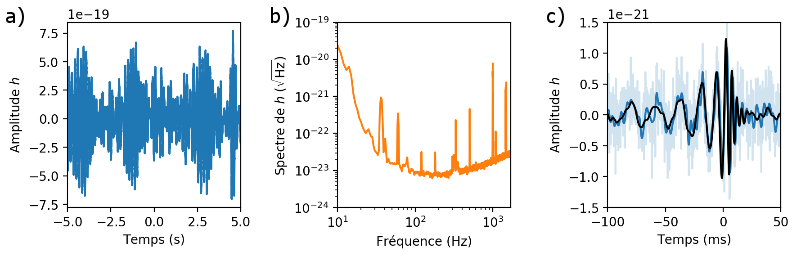
\includegraphics[scale=0.75]{figures/GW150914_data.png}
\caption{Filtrage numérique des données brutes de l'interféromètre gravitationnel LIGO situé à Hanford pour extraire le signal associé à l'évènement GW150914.
Il s'agit de la première observation directe d'ondes gravitationnelles issues de la coalescence de deux trous noirs.
Les données brutes (a) sont largement dominées par des bruits basse fréquence.
Le passage dans l'espace de Fourier (b) permet d'identifier et d'atténuer les raies spectrales propres à l'appareil : \unit{60}{\hertz} du secteur américain, vibrations mécaniques, etc.
Finalement, le lissage des données par un filtre passe-bas qui peut être implémenté par les étudiants permet d'obtenir le signal historique (c).
La courbe noire correspond au modèle théorique dont sont extraits les paramètres de la source des ondes gravitationnelles.}
\label{fig:GW150914}
\end{figure}

L'expérience dépend de nombreux filtres et d'amplificateurs analogiques et numériques.
J'ai notamment réalisé des filtres électroniques passifs et actifs, des photodiodes à haute efficacité quantique et faible bruit et un contrôleur fondé sur une carte Arduino interfacé avec Python permettant le positionnement reproductible d'une translation motorisée.
Le bon déroulement de nos mesures repose également sur plusieurs boucles de rétroaction : stabilisations de températures, de puissances optiques et asservissement de longueur portant sur la position des miroirs des cavités et interféromètres.
Les asservissements sont pour la plupart réalisés numériquement par des micro-contrôleurs RedPitaya et la bibliothèque \textit{open source} PyRPL\footnote{\url{https://pyrpl.readthedocs.io/en/latest/}} (Python RedPitaya Lockbox) développée au sein de l'équipe.
Il est ainsi possible de piloter une grande partie de l'expérience à partir d'un PC, ce qui permet l'automatisation des séquences de mesures grâce à un répertoire de scripts Python que j'ai progressivement étoffé.

Je mettrai à profit ces compétences par exemple avec des étudiants en PSI lors d'un TP pour la réalisation du filtrage d'un signal.
Dans un premier temps, le signal généré par un micro-contrôleur et constitué d'une sinusoïde de faible amplitude masquée par un bruit blanc sera filtré analogiquement à l'aide d'un circuit RLC réalisé par les étudiants dont la bande-passante devra être caractérisée et optimisée.
Ensuite, ils numériseront convenablement le signal grâce à un oscilloscope, son spectre sera analysé en utilisant la FFT, et la composante harmonique pourra être isolée grâce à des filtres numériques implémentés en Python par les étudiants.
Finalement, je montrerai la puissance du filtrage numérique en l'appliquant sur les données des interféromètres gravitationnels LIGO et Virgo (Fig.~\ref{fig:GW150914}).
Elles sont disponibles publiquement\footnote{\url{https://www.gw-openscience.org/GW150914data/GW150914_tutorial.html}} et peuvent être exploitées en suivant les guides rédigés par la communauté.
J'évaluerai aussi leur compréhension des similitudes entre filtrage électronique et mécanique en les questionnant sur le rôle des suspensions des miroirs de Virgo dans l'isolation des bruits sismiques.

\subsubsection{Un interféromètre de Michelson imprimé en 3D}

L'impression 3D devient de plus en plus incontournable.
À plusieurs reprises au cours de ma thèse, j'ai eu recours à cet outil qui permet de créer rapidement des composants entièrement personnalisés et d'éprouver des assemblages complexes avant d'en réaliser des versions plus permanentes.
Cette technologie sera mise à profit dans le cadre du projet expérimental et numérique de l'enseignement scientifique de première ou auprès d'associations d'élèves reproduisant le fonctionnant des actuels fablab.
Si l'établissement n'en dispose pas, je souhaite proposer leur acquisition auprès du conseil d'administration si les budgets le permettent.

Notre équipe a développé un interféromètre de Michelson dont les montures mécaniques sont imprimées en 3D.
La longueur d'un bras est contrôlée grâce à une bobine et une monture déformable aimantée semblable à une membrane de haut-parleur.
Les miroirs sont des morceaux de mosaïque métalisée, la source lumineuse une diode laser et l'interféromètre est piloté à l'aide d'un Arduino.
Seule la séparatrice est de qualité optique et l'ensemble coûte moins de 100\,\euro.
L'interféromètre peut être construit par les élèves ou imprimé dans un fablab local.

J'exploiterai l'interféromètre dans le cadre d'un classe de terminale S lors de l'étude des propriétés des ondes, sans bien sûr rentrer dans les subtilités de l'appareil.
Les élèves réaliseront tout d'abord une simulation numérique pour comprendre l'effet d'un déphasage sur la superposition de deux ondes.
Ils produiront ensuite un signal sinusoïdal à l'aide de l'Arduino et s'en serviront pour moduler la longueur d'un bras de l'interféromètre.
Il pourront alors mesurer les variations de l'intensité à la sortie de l'interféromètre et rapprocher leurs observations des simulations. 

\subsection{Enseignements}

Au cours de ma thèse, j'ai effectué une mission d'enseignement qui m'a donné l'occasion de mettre en pratique plusieurs approches de l'enseignement.
L'unité d'enseignement de physique expérimentale est certainement celle qui m'a le plus apporté.
Cette UE ne contient aucun cours magistral et se compose d'une série de TP abordant l'électronique numérique et analogique ainsi que la programmation (Labview).
Chaque séance de TP est précédée d'un TD dont l'objectif est surtout de présenter aux étudiants le matériel qu'ils devront utiliser et d'aborder les concepts nouveaux en se basant sur des observations expérimentales.
Les TP les confrontent ensuite à des objectifs concrets, comme la réalisation d'un bras capable de détecter et saisir un objet, où ils doivent exploiter et se familiariser avec ces nouveaux concepts.
Ils disposent enfin d'une grande liberté pour l'objectif de fin de semestre, une compétition de robots : combats de \og sumos\fg{}, positionner un drapeau au plus près d'une cible, etc.

Le parcours des étudiants que j'ai pu encadrer est souvent très disparate et il m'a parfois été difficile de m'adapter à chacun.
Leur investissement était toutefois réel et les séances très interactives.
Cette approche par l'expérience me semble essentielle puisqu'elle amène les étudiants à se poser eux-même les questions grâce auxquelles ils apprennent des notions nouvelles.
La nature même de ma thèse, profondément expérimentale, renforce cette conviction puisqu'elle m'a permis d'acquérir de nombreuses compétences et de consolider mes connaissances théoriques dans plusieurs domaines.
C'est une méthode d'enseignement très vivante que je mettrai en œuvre : l'exploitation d'expériences, y compris durant les cours, me semble essentielle pour ancrer le discours dans une réalité quotidienne ou une actualité scientifique.

\subsection{Vulgarisation : résonance et ondes gravitationnelles}

À l'occasion du sujet \textit{Peut on casser un verre avec la voix ?} de l'émission E=M6, j'ai aussi mis en place une expérience permettant de casser un verre en le faisant vibrer à l'aide d'un haut-parleur.
%\footnote{\url{https://youtu.be/7cgZcbHmxm4}}
Dans le cadre de l'objectif thématique sur le son de l'enseignement scientifique de première, les élèves pourront visualiser le spectre du son émis par un verre vibrant.
Une analogie avec la corde vibrante permet de discuter qualitativement de la fréquence fondamentale et la présence des harmoniques expliquée par l'existence de différents modes propres (Fig.~\ref{fig:wine_glass}).
Le transport d'énergie par les ondes acoustiques sera mis en évidence en le faisant vibrer grâce à un haut parleur.
Dans cette expérience, on observe les vibrations du verre avec un éclairage stroboscopique réalisé à partir d'un GBF ou d'un Arduino par exemple.

Le sujet de ma thèse, son contexte et mon intérêt pour la diffusion de connaissances m'ont aussi amené à plusieurs reprises à des activités de médiation auprès de publics très variés.
L'actualité récente depuis fin 2015 autour des ondes gravitationnelles a mis en avant les travaux liés à leur détections et à l'implication de telles observations.
La communauté LIGO/Virgo est très dynamique et offre des ressources qu'il est possible de réinvestir à tous les niveaux.
Par exemple, avec les connaissances des étudiants en PCSI sur les systèmes à force centrale et quelques hypothèses, il est possible d'analyser l'allure du signal détecté lors de l'évènement GW150914\footnote{Mathur \textit{et al.}, An Analysis of the LIGO Discovery based on Introductory Physics, \textit{Am. J. Phys.}, (2017)}.
J'ai réalisé des présentations sur la détection des ondes gravitationnelles devant des lycéens à l'occasion des Olympiades de physique, des fêtes de la Science organisées à Jussieu (Sorbonne Université), devant le personnel technique et administratif du LKB et finalement au Palais de la Découverte pour l'exposition \textit{Un chercheur, Une manip}.
La préparation, la présentation et les échanges qui ont suivi ces présentations ont été autant d'occasions de s'approprier différents aspects liés à ce thème, mais aussi d'expérimenter différentes approches afin de faire passer au mieux mon message en m'adaptant à l'auditoire.
Ce sujet, par la variété des domaines qu'il fait intervenir, peut servir de fil conducteur et permettra de rattacher les sujets abordés en cours à une actualité scientifique qui promet de nombreux rebondissements.


\begin{figure}[b]
\center
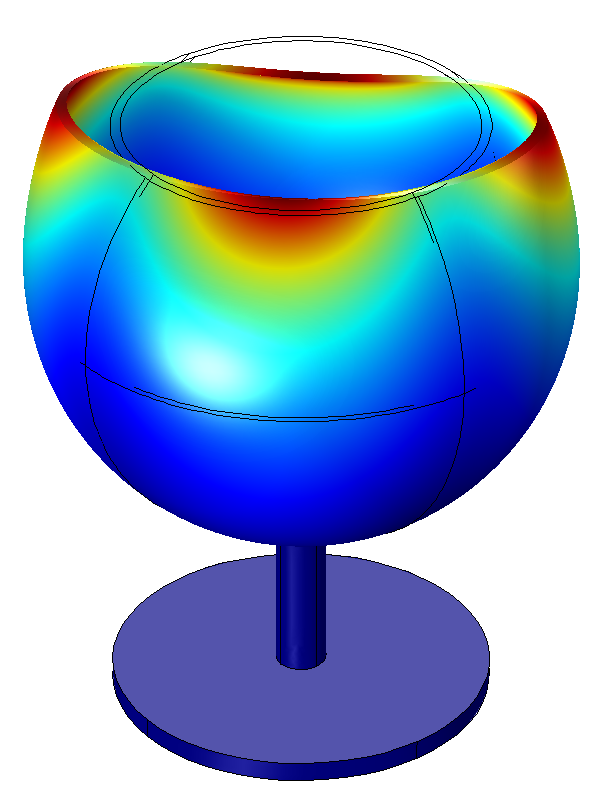
\includegraphics[height=100pt]{figures/wine_glass_f0.png}
\hfill
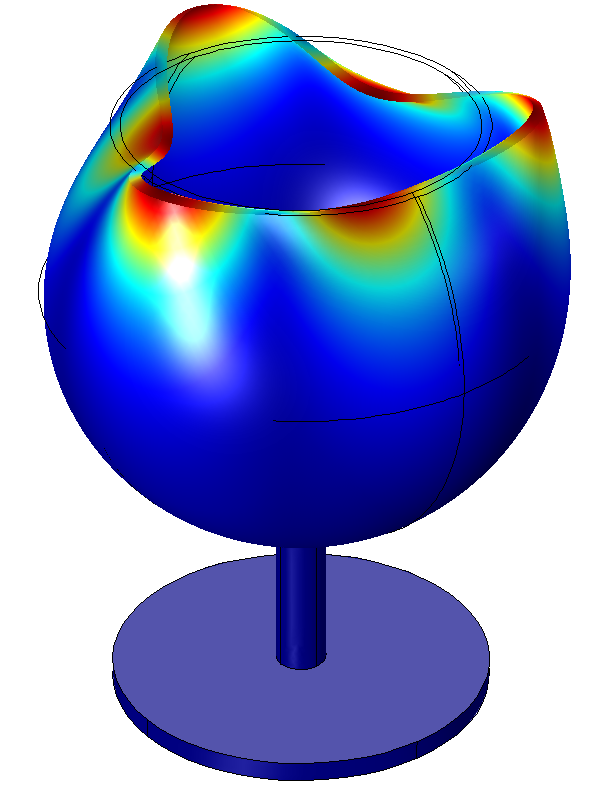
\includegraphics[height=100pt]{figures/wine_glass_f1.png}
\hfill
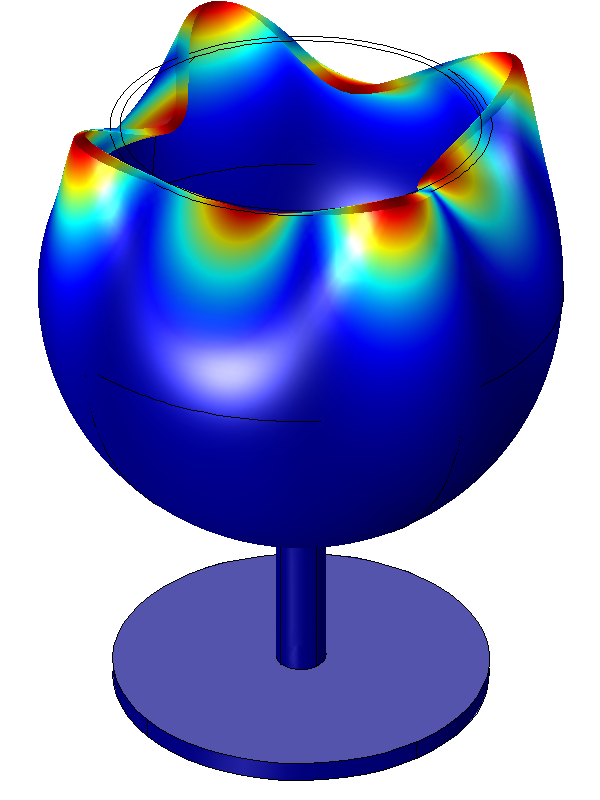
\includegraphics[height=100pt]{figures/wine_glass_f2.png}
\hfill
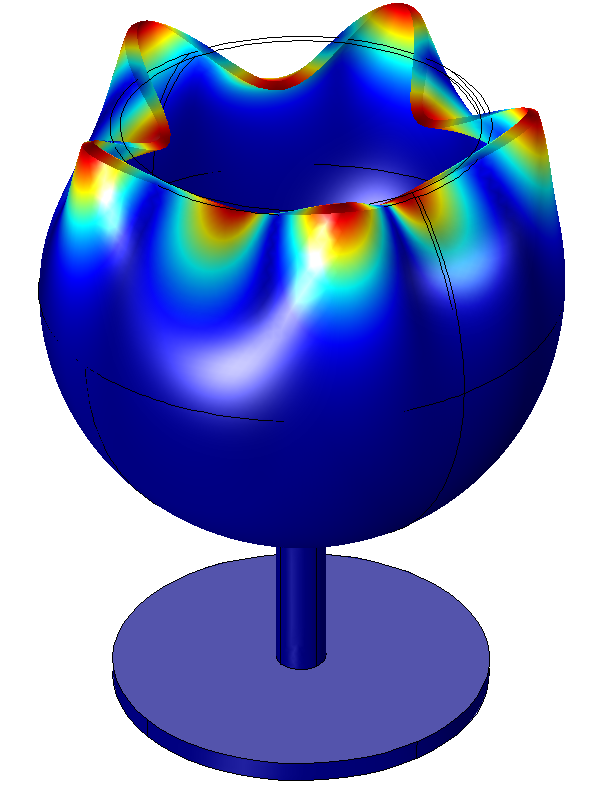
\includegraphics[height=100pt]{figures/wine_glass_f3.png}
\hfill
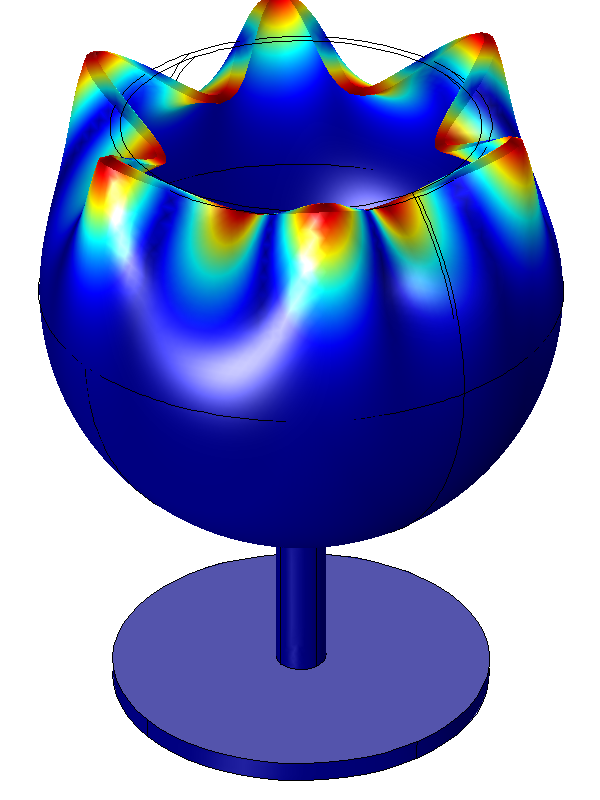
\includegraphics[height=100pt]{figures/wine_glass_f4.png}
\caption{Simulations par élément fini des premiers modes propres mécaniques d'un verre.}
\label{fig:wine_glass}
\end{figure}

\end{document}